
\subsection{Authentication Robustness of \systemname} After evaluating the authentication accuracy of \systemname~, we next study how robust it is against intentional imitation. For this purpose, we asked a number of subjects (imitators) to imitate simple nodding movements from three subjects (imitatees) after watching the imitatee's movement video for as long as they desire, and reported their chances of successful imitation. We note that the nodding movements are the simplest head-movement patterns and easiest to be imitated; hence, the results presented here outline the \emph{lowest} robustness that \systemname~offers. In reality, users are more likely to employ more sophisticated head-movement patterns, which will lead to much better robustness.

\subsubsection{Participants}
We had total of 38 volunteer participants. The participants list included a total of 32 males and 6 females.
The average age of the participants was 25.6 years with a standard deviation
of 6.6 years. The youngest participant was 22 years old while the eldest was
at 49 years.
\subsubsection{Procedure}
Our second experiment aimed at an practical imitation attack field test scenario. In this experiment, three subjects were taken video while they were performing their successful login movement. Note that the music cue is usually played via a bone conduction speaker or a earplug, hence a camcorder is difficult to capture the music sound if the environment is noisy or the microphone is not sensitive enough. In this case, the imitators will be impossible to synchronize the music with the video. To eliminate this concern, we set the volume of the speaker to maximum and took the video in a quiet laboratory environment.

The participants were divided into three group, and each group was asked to imitated only one of the three users above. During the test, the participants could watch the video for as many time as their willing at anytime between two trials. A feedback from our system would be provided after each trail so that the participants could decide whether they needed to adjust their movement or not. After total number of trials reached 30 for each participant, the experiment would stop regardless the participant succeed or not. The investigator was not only recording the total number of successes, but also the number of trail before the first successful login. This experiment was conducted in quite space on campus. We will now discuss our evaluation results for both experiments in detail.

\subsubsection{Results}
Although it is difficult to quantitatively to describe the complexity of the movement in 5-Dimension space(3-axis accelarometer, time space,  and response to the music beat), there are some distinguish characteristics of these three subjects, hence they are chosen to become our imitated subjects. As shown in Figure~\ref{fig:imitation_movement} $Subject A$ performed a simple nodding movement by naturally following the music flow. $Subject B$ also performed a simple nodding, but his movement was always off-beat with the music. $Subject C$ performed a movement combined with nodding and shaking, and he only nodded/shake at certain beats instead of every beat, which makes his movement is relatively difficult to learn. Table~\ref{tab:imitation} shows the overall result of this experiment. The overall FAR is 7.54 \%, while the individual FARs are 17.67\%, 9.82\% and 3.27\% accordingly.  Since $Subject A$ perform the simplest movement among these three subjects, 6 out 10 subjects could succeed at least once during their 30 trials, while for $Subject B$ and $Subject C$ this number is 3 of 15 and 3 of 10.

\begin{table}[]
\centering
\label{my-label}
\begin{tabular}{lcccc}
\hline
                            & \multicolumn{1}{l}{Total Imitator} & \begin{tabular}[c]{@{}c@{}}Successful Imitator \\ Number\end{tabular} & \begin{tabular}[c]{@{}c@{}}Average Number of \\ Trial before \\ First Successful Login\end{tabular} & \multicolumn{1}{l}{FAR (\%)} \\ \hline
Subject A                   & 12                                 & 7                                                                     & 10.33                                                                                               & 15.83                        \\ \hline
Subject B                   & 13                                 & 3                                                                     & 14.33                                                                                               & 2.77                         \\ \hline
Subject C                   & 12                                 & 3                                                                     & 17.67                                                                                               & 2.72                          \\ \hline
\multicolumn{1}{c}{Overall} & 38                                 & 13                                                                    & 13.17                                                                                                    & 6.94                         \\ \hline
\end{tabular}
\caption{\label{tab:imitation}Imitation attack experiment result. Successful Imitator Number represents the number of the imitators that succeed at least once. Average Number of Trail before first login indicates the average times of trail a successful imitator takes before the first login.}
\end{table}



\subsection{Headbanger Google Glass App Implementation}\label{subsec:app}

\begin{figure}[t]
\centering
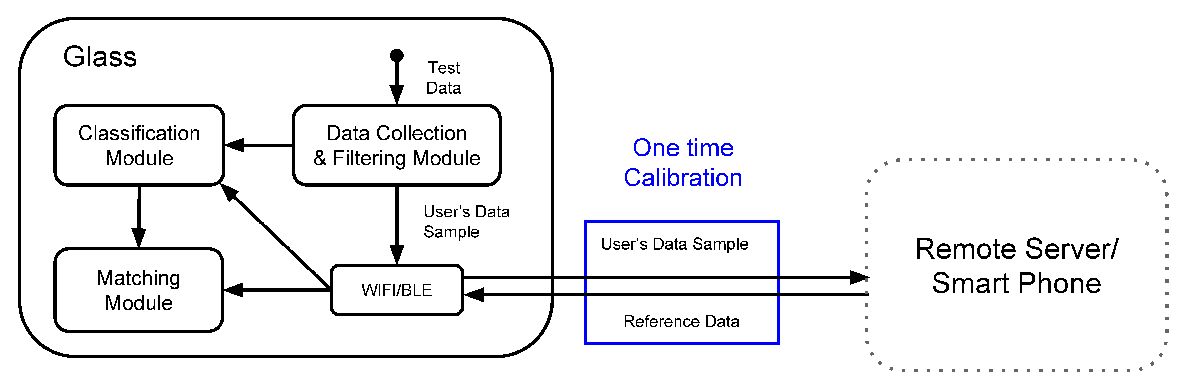
\includegraphics [width=\columnwidth]{figure/software_arch.eps}
\caption{Software modules of \systemname~implementation}
\vspace{25 pt}
\label{fig:glass-softwarearch}
\end{figure}

We implemented \systemname~on Google glass, positioning it as an
authentication application (app).
Figure~\ref{fig:glass-softwarearch} shows the main software modules in the
app. Upon initiation by the user, the app plays a music cue for a stipulated
duration. The user conducts head-movements in synchrony with the music cue
while the app records the accelerometer sensor in parallel. At the end of the
music cue duration the app executes the data processing phase where the
sensor readings are input to the \systemname's software modules for
processing. The processing stage includes the filtering of the accelerometer
sensor values, classification and feature extraction using DTW, and threshold
based matching of the generated features with those from training set.
%\systemname extracts the head-movement features through
%the thresholding process discussed in section~\ref{sec:design}, and compare
%with the feature templates generated from the training phase.
Upon completion of data processing, the app responds with a YES or NO textual
output on the Google Glass screen, depending on match score.

In our current implementation, the training phase is conducted offline, prior
to live-testing off the application.
The training phase involves collecting 30 samples (variable) of the
head-movement accelerometer readings, generating the features, and saving them
into a local server (running on PC) as an XML file, with appropriate indexing.
Upon app initiation on Glass, the trained features are pre-fetched from
the server through a wireless connection. This ensures that the training set
is readily available during the authentication process, thus eliminating the
additional processing time required for the training phase.
Conducting online training, particularly that involves DTW computations, is
very compute intensive on a resource constrained devices such as Glass.
One possible solution would be for the Glass to offload the
training phase computation to a local server machine.
%We reserve such considerations for future implementations.

%Among all the software modules, the ``training set construction model'' is
%the most computing-intensive, and as a result, we executed the model on the
%bluetooth-paired smartphone. The rest of the modules are implemented and
%executed on the glass.
%In our on-glass app, the classification module runs the
%thresholding-based classification.
\subsubsection{Response time}

\begin{table}
\centering
\begin{tabular}{|ccclc|}
\hline
\multicolumn{1}{|c|}{\multirow{2}{*}{\begin{tabular}[c]{@{}c@{}}music  cue \\
duration (s)\end{tabular}}} &
\multicolumn{1}{c|}{\multirow{2}{*}{\begin{tabular}[c]{@{}c@{}} response\\
time (s)\end{tabular}}} & \multicolumn{3}{c|}{time breakdown (\%)}
\\ \cline{3-5}
\multicolumn{1}{|c|}{}
                             &
\multicolumn{1}{c|}{}
                              &
 Filtering & \multicolumn{1}{c}{DTW} & Thresholding   \\
 \hline\hline
10
                             &
1.93
                              &
 0.50      & 99.50                   & \textless0.01  \\
6
                             &
1.15
                              &
 0.64      & 99.36                   & \textless0.01  \\
5
                             &
0.88
                              &
 0.81      & 99.19                   & \textless0.01 \\ \hline
\end{tabular}
\caption{\label{tab:glass} Measured response time of \systemname~app implementation on Google
Glass with different music cue durations and for $K = 1$. The response time
reported here is an average over 20 trials.}

\end{table}

In Table~\ref{tab:glass} we report the measured average response-time
of the \systemname implementation on Google Glass app for music cue durations
of 5,6 and 10 seconds. We conducted the benchmark execution-time profiling of
\systemname~on Glass in a controlled indoor laboratory setting with no
mobility. We define response time as the time elapsed between music cue
completion to
the display of authentication response (YES/NO text) on the Glass screen.
Our measurements indicate that the response time is within 5 seconds for a 10
second data input, and is almost halved for a 5 second data input.
We feel that a response time of 2-5 sec for a local authentication solution in
Google Glass is comparable to that of prior-art that comes close to our
solution~\cite{von2013patterns,egelman2014you}.
It is also important to note that authentication solutions that execute
locally on head-worn wearable devices, especially on a heavily resource
constrained device like Glass, are still not mature. However, the hope is that
such solutions will possibly catch up to speed in the near future and that our
approach is advancing one step in that direction.
In Table~\ref{tab:glass} we also report the execution time of the key
processes in \systemname; filtering, DTW computation ($K = 1$ requires 1 DTW
computation), thresholding based similarity matching.
We can observe from Table~\ref{tab:glass} that the DTW computation
dramatically compute intensive than the other processes.

It is important to note that our current implementation uses a faster
version of the DTW algorithm called Fast DTW~\cite{salvador2007toward},
providing about 2x speed-up in DTW computation.
We believe that the response time can be reduced
further through strategic methods such as, further optimizations in the Fast
DTW algorithm or pipelining the app execution along with data collection.
A specific strategy for reducing response time for rejected attempts can be
that, after a short duration, before the entire music cue is played, if it is
found that a user's movement does not match the signature of the claimed user
with a sufficient pre-determined confidence level, then the on-site
classification may be terminated instead of waiting for the entire duration to
yield the rejection.
Another example, may include cyber-foraging strategies to offload heavy
computation tasks, such as online training and classification, to the user's
Bluetooth paired smartphone or a nearby cloudlet~\cite{ha2014towards}.

